% ============================================================================
% SECTION 1: INTRODUCTION (CONCISE - Compressed from 1.5 to 1.0 pages)
% ============================================================================

\section{Introduction}
\label{sec:introduction}

Large language models have created unprecedented opportunities for creative and analytical work, yet access remains concentrated among those with substantial budgets or ML expertise. Frontier models (GPT-4o, Claude-3.5-Sonnet) cost \$4--15 per 1,000 queries at late-2024 on-demand prices~\cite{openai2025pricing,anthropic2025pricing}, creating \emph{economic barriers} that exclude students, independent researchers, and resource-constrained startups. While the ecosystem has fragmented into more than 80 specialized models offering comparable quality at \$0.10--0.88 per 1,000 queries (snapshot as of December 2024)~\cite{openrouter2025models,artificialanalysis2025}, practitioners face \emph{expertise barriers}: existing routing tools require hundreds to thousands of labeled examples for calibration in typical deployments~\cite{chen2023frugalgpt}, domain-specific scorer training, and nontrivial setup time. These dual barriers result in systematic over-provisioning (users default to expensive models) or abandoned optimization entirely.

Existing solutions address one barrier while perpetuating the other. FrugalGPT~\cite{chen2023frugalgpt} reduces costs via cascading chains but requires extensive offline profiling and expert-designed scoring functions. RouteLLM~\cite{ong2024routellm} simplifies binary routing but relies on thousands of preference pairs and classifier retraining when models evolve. Semantic routers (e.g., Aurelio~\cite{aureliolabs2024semantic}) offer deterministic control but require manual intent definitions that are brittle as model capabilities evolve or new domains emerge. As illustrated in Figure~\ref{fig:deployment_comparison}, traditional routers require days-to-weeks of offline calibration (data collection, benchmarking, retraining), creating an operational bottleneck that confines adaptive routing to specialized teams with ML infrastructure. The central challenge: \textit{Can we achieve cost-efficient routing with operational simplicity accessible to non-experts?}

\begin{figure}[t]
    \centering
    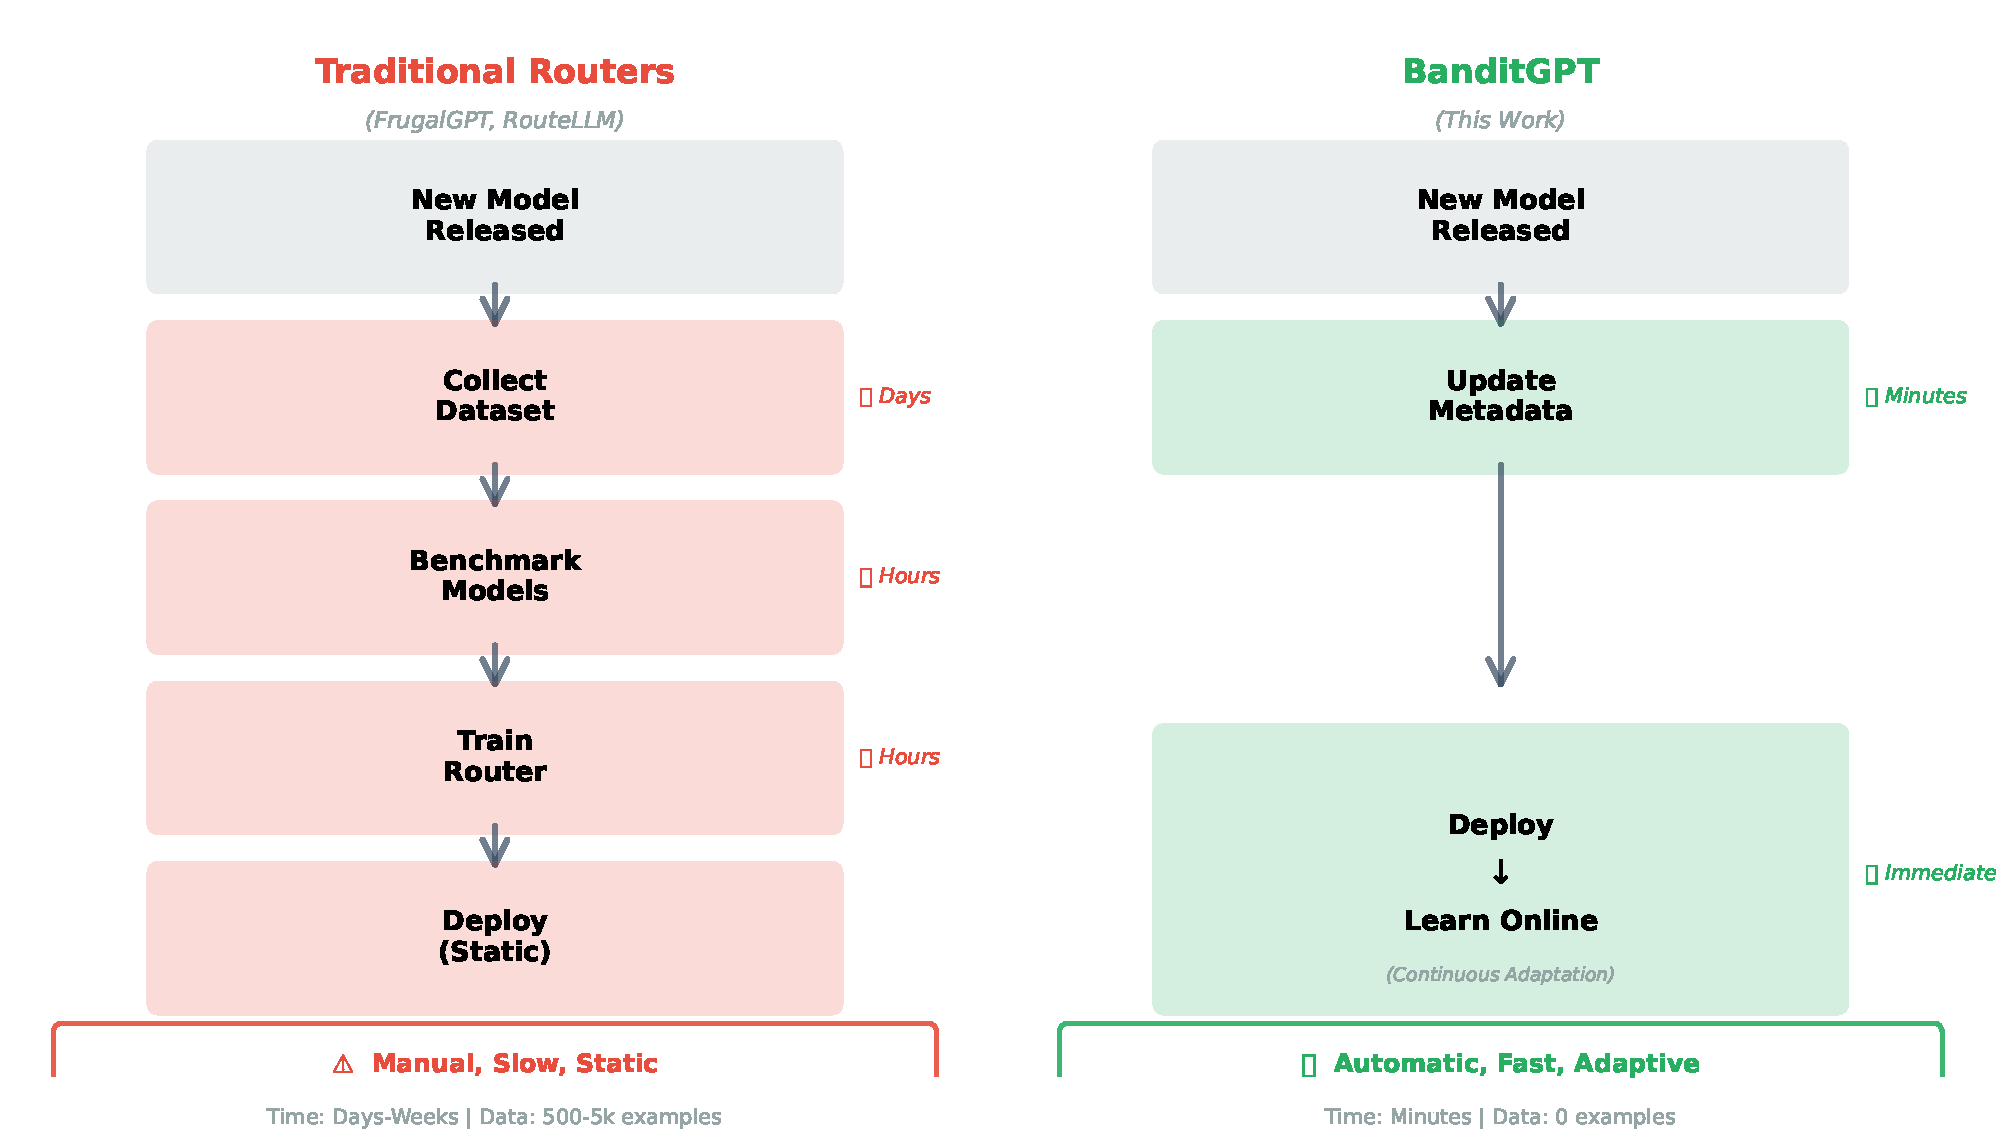
\includegraphics[width=\columnwidth]{figures/figure1_deployment_comparison/figure1_deployment_comparison.pdf}
    \caption{\textbf{Deployment Workflow Comparison.} Traditional LLM routers (e.g., FrugalGPT, RouteLLM) require days-to-weeks of offline calibration, including dataset collection (500-5000 examples), benchmarking, and retraining. **BanditGPT eliminates this bottleneck** through pure online learning, enabling immediate deployment without training data. When model capabilities change, traditional routers require manual recalibration, while BanditGPT adapts automatically through continuous feedback.}
    \label{fig:deployment_comparison}
\end{figure}

\paragraph{Our Approach: Deploy and Learn.}
We present \ours{}, an open-source framework that removes both barriers through three innovations: \textbf{(1) Pure online learning}---deploying immediately without training data and converging to optimal routing within $\sim$200 interactions. Through rigorous 5-fold cross-validation, we show that offline calibration on <1K prompts exhibits consistent negative transfer (+32\% regret), validating zero-calibration deployment. \textbf{(2) Zero-benchmark model addition}---users register new models in 30 seconds; the bandit autonomously learns their strengths via online exploration (vs.\ 1--3 days of offline profiling). \textbf{(3) Intuitive constraint interfaces}---users specify \texttt{max\_budget}, \texttt{min\_quality}, \texttt{max\_latency} rather than ML hyperparameters, enabling non-technical decision-makers to control routing.

\paragraph{Evaluation and Impact.}
Experiments on 2,000 real-world prompts across 81 production models demonstrate: \textbf{Limits of offline calibration} (\S\ref{sec:rq1})---through rigorous 5-fold cross-validation, we show that warm-start strategies on <1K calibration prompts exhibit consistent negative transfer (Shared: +32\% regret, Disjoint: +27\%, 100\% fold consistency), establishing sample complexity bounds and validating metadata-guided cold start. \textbf{Cost-quality frontier} (\S\ref{sec:rq3})---standard mode achieves \$0.70 per 1k queries (61\% cheaper than FrugalGPT's \$1.78) with zero calibration; hybrid mode delivers 98\% reliability across 80+ models without manual chain design. \textbf{Operational simplicity}---routing overhead is 8.94ms P99 (1.1\% of latency); adding new models requires 30 seconds (vs.\ days); constraints specified via intuitive parameters.

By eliminating calibration requirements and providing accessible control interfaces, we expand adaptive routing from ML specialists (requiring labeled datasets and domain expertise) to general programmers (requiring basic Python skills), increasing the addressable user base by roughly an order of magnitude ($\approx 15$--$25\times$)~\cite{stackoverflow2024survey,github2025developer}. Our work demonstrates that democratizing AI access requires addressing not only cost, but the operational complexity that confines proven techniques to specialized teams.

\paragraph{Contributions.}
\begin{itemize}[leftmargin=*,nosep]
    \item \textbf{Pure online learning architecture} enabling zero-calibration deployment that converges within $\sim$200 interactions without training data.
    \item \textbf{Scientific insight: limits of offline calibration.} Through rigorous 5-fold cross-validation, we demonstrate consistent negative transfer (+32\% regret, 100\% fold consistency) on <1K calibration prompts, identifying two failure mechanisms (Herd Suppression, Overfitting) and establishing sample complexity bounds.
    \item \textbf{Zero-benchmark model addition} enabling users to track market evolution via 30-second registration without offline profiling.
    \item \textbf{Intuitive constraint interfaces} democratizing control through domain terms (\texttt{max\_budget}, \texttt{min\_quality}) rather than ML hyperparameters.
    \item \textbf{Empirical validation} demonstrating 61--84\% cost reduction while maintaining 95--98\% accuracy across 2,000 prompts and 81 models.
    \item \textbf{Open-source release} expanding adaptive routing from ML specialists to general practitioners.
\end{itemize}


